%%%%%%%%%%%%%%%%%%%%%%%%%%%%%%%%%%%%%%%%%%%%%%%%%%%%%%%%%%%%%%
% --> INTRODUCCIÓN
%%%%%%%%%%%%%%%%%%%%%%%%%%%%%%%%%%%%%%%%%%%%%%%%%%%%%%%%%%%%%%
\section{Introducción}


%%%%%%%%%%%%%%%%%%%%%%%%%%%%%%%%%%%%%%%%%%%%%%%%%%%%%%%%%%%%%%
% --> OBJETIVOS
%%%%%%%%%%%%%%%%%%%%%%%%%%%%%%%%%%%%%%%%%%%%%%%%%%%%%%%%%%%%%%
\subsection{Objetivos}



%%%%%%%%%%%%%%%%%%%%%%%%%%%%%%%%%%%%%%%%%%%%%%%%%%%%%%%%%%%%%%
% --> OBJETIVO GENERAL
%%%%%%%%%%%%%%%%%%%%%%%%%%%%%%%%%%%%%%%%%%%%%%%%%%%%%%%%%%%%%%
\subsubsection{Objetivo General}
\begin{itemize}
\item 
\end{itemize}

%%%%%%%%%%%%%%%%%%%%%%%%%%%%%%%%%%%%%%%%%%%%%%%%%%%%%%%%%%%%%%
% --> OBJETIVOS ESPECÍFICOS
%%%%%%%%%%%%%%%%%%%%%%%%%%%%%%%%%%%%%%%%%%%%%%%%%%%%%%%%%%%%%%
\subsubsection{Objetivos Específicos}
\begin{itemize}
\item 
\item 
\item 
\item
\item 
\end{itemize}

%%%%%%%%%%%%%%%%%%%%%%%%%%%%%%%%%%%%%%%%%%%%%%%%%%%%%%%%%%%%%%
% --> ENUNCIADO
%%%%%%%%%%%%%%%%%%%%%%%%%%%%%%%%%%%%%%%%%%%%%%%%%%%%%%%%%%%%%%
%\newpage

%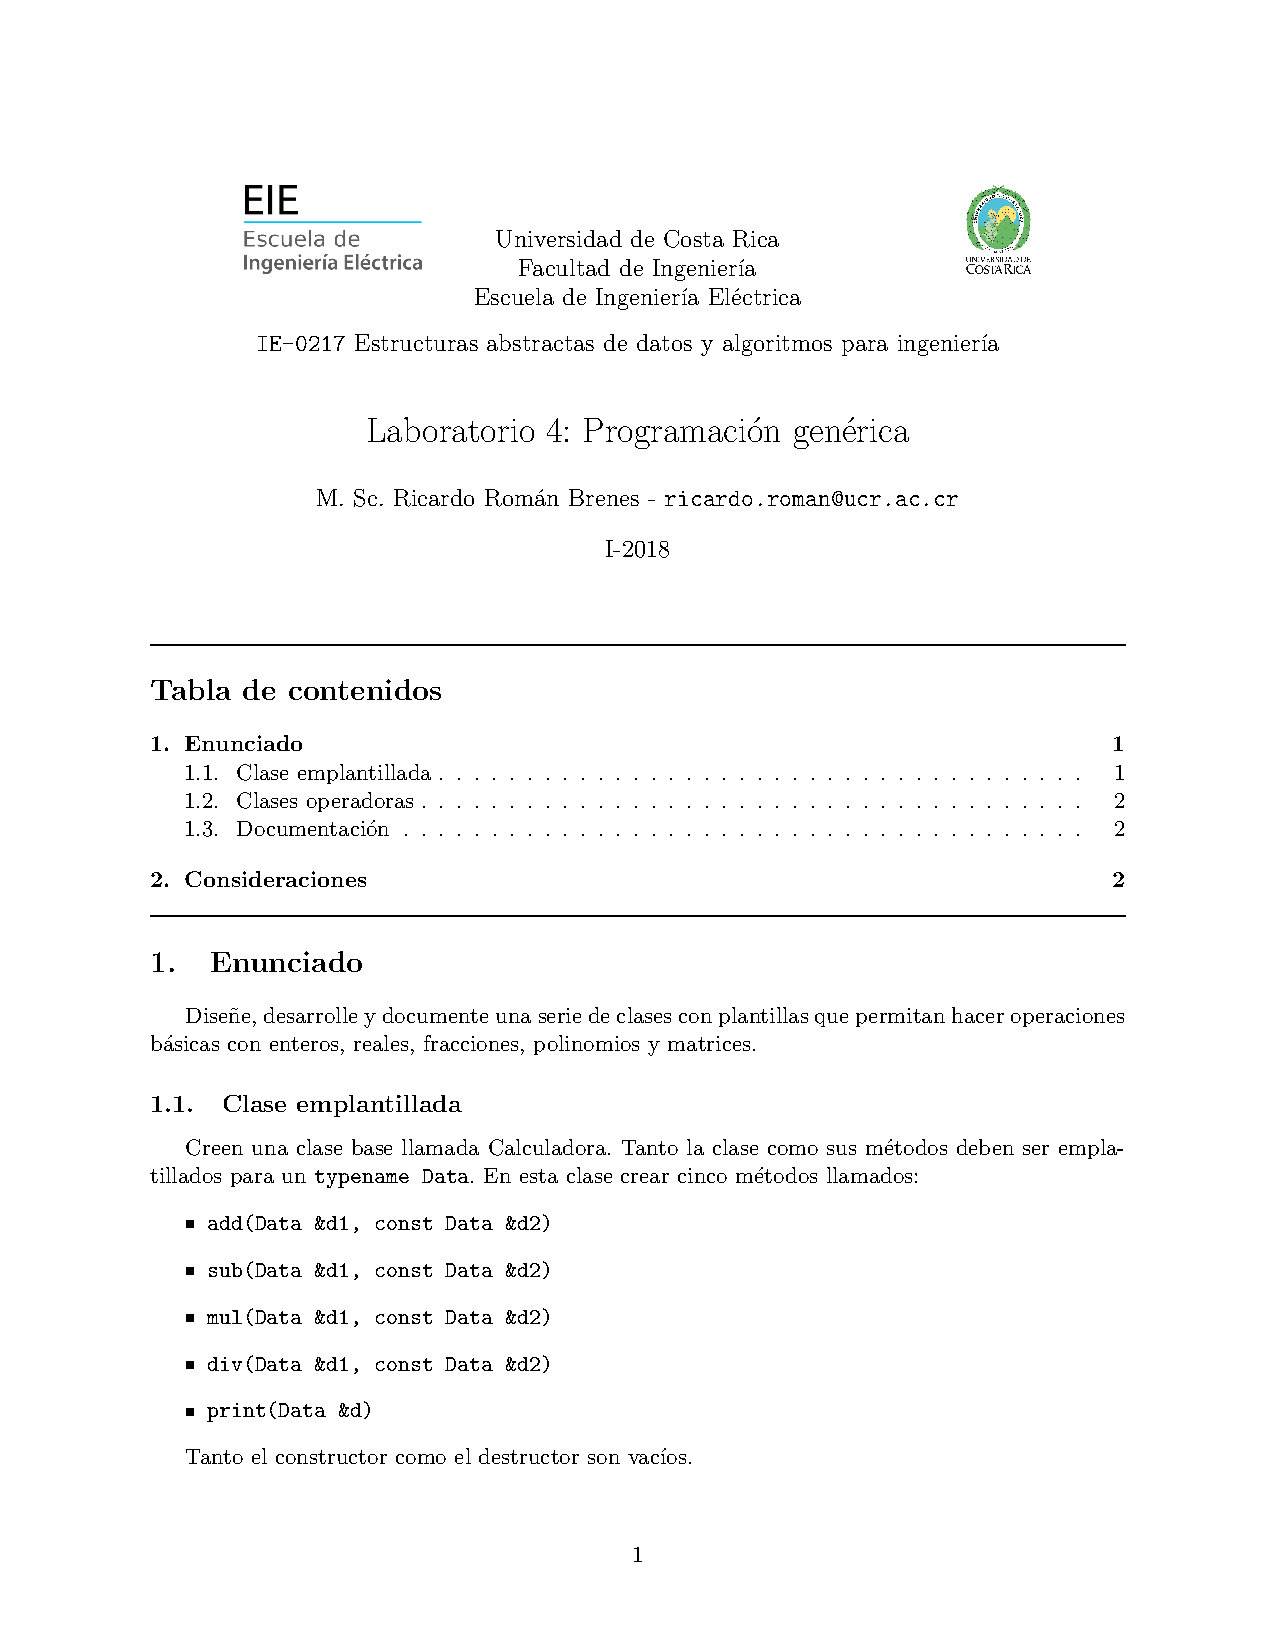
\includepdf[pages=1,pagecommand=\section{Enunciado}, scale=0.8]{enunciados/enun4} 
%\includepdf[pages=2,pagecommand={},scale=0.8]{enunciados/enun4}

%%%%%%%%%%%%%%%%%%%%%%%%%%%%%%%%%%%%%%%%%%%%%%%%%%%%%%%%%%%%%%
% --> SOLUCIÓN
%%%%%%%%%%%%%%%%%%%%%%%%%%%%%%%%%%%%%%%%%%%%%%%%%%%%%%%%%%%%%%
\section{Solución}


\begin{minted}[linenos,autogobble,bgcolor=bg,breaklines,fontsize=\footnotesize ]{c++}
#include <string>
#include <iostream>
using namespace std;

class FileUtil
{
  public:
  	FileUtil(string s, ios_base::openmode p);
  	~FileUtil();
  	string read();
  	string* readLines();
  	int write(string s);
  	int write(string* s, int n);
    void countNumberLines();
    int getNumberLines();
  private:
    //Numero de lineas.
    int numLines;
    //Dirección de lectura.
    string ruta;
    //Modo de lectura.
  	ios_base::openmode modo;
    //Linea leida.
    string line;
    //Puntero con la direccion del arreglo de las lineas leidas.
    string* lines;

};
\end{minted}



%%%%%%%%%%%%%%%%%%%%%%%%%%%%%%%%%%%%%%%%%%%%%%%%%%%%%%%%%%%%%%
% --> RESULTADOS
%%%%%%%%%%%%%%%%%%%%%%%%%%%%%%%%%%%%%%%%%%%%%%%%%%%%%%%%%%%%%%
\section{Resultados}



%%%%%%%%%%%%%%%%%%%%%%%%%%%%%%%%%%%%%%%%%%%%%%%%%%%%%%%%%%%%%%
% --> CONCLUSIONES
%%%%%%%%%%%%%%%%%%%%%%%%%%%%%%%%%%%%%%%%%%%%%%%%%%%%%%%%%%%%%%
\section{Conclusiones}


Como conclusiones se tiene que:

\begin{itemize}
\item 
\item 
\item 
\item 
\end{itemize}


%%%%%%%%%%%%%%%%%%%%%%%%%%%%%%%%%%%%%%%%%%%%%%%%%%%%%%%%%%%%%%
% --> BIBLIOGRAFIA
%%%%%%%%%%%%%%%%%%%%%%%%%%%%%%%%%%%%%%%%%%%%%%%%%%%%%%%%%%%%%%
\begin{thebibliography}{IEEE}
\bibitem{R1} Talens, S. \textbf{\textit{Curso de programación en C++}}. EUI (UPV) Valencia, 17 al 28 de Julio de 1995. 

\bibitem{R2} Raffo, E. \textbf{\textit{Programación genérica en C++, usando Metaprogramación}}. 2007. Sistemas de Informática. 
\end{thebibliography}

